\documentclass[convert = false, tikz]{standalone}
\usepackage[utf8]{inputenc}
\usepackage{tikz}
\usepackage{adjustbox}
\usepackage{txfonts}
\usetikzlibrary{automata, positioning, arrows, fit}
 
% arara: pdflatex
% arara: latexmk: { clean: partial }
\begin{document}
    \tikzset{
    every state/.style={draw=none, text centered, align=center, inner sep=1mm}, % sets style for all states
    }
    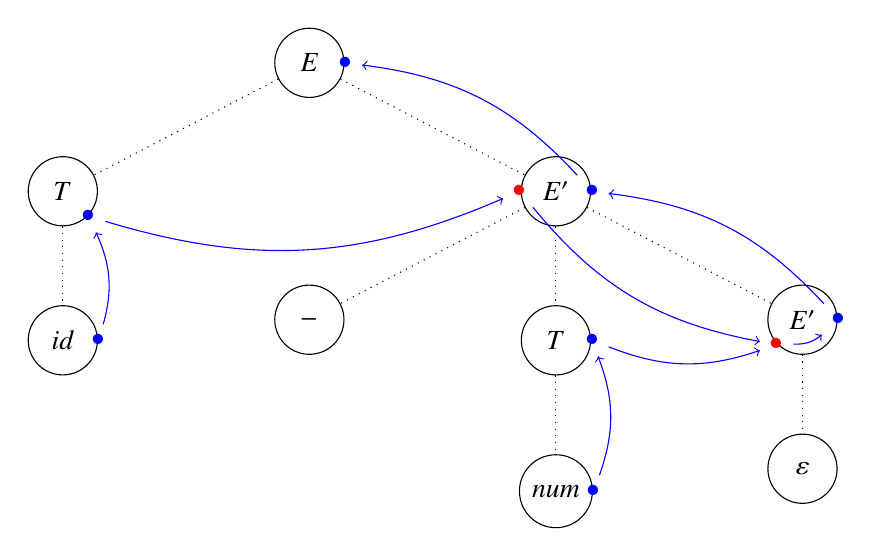
\begin{tikzpicture}[node distance=1cm and 2.5cm]
        % First level
        \node[state] (a) {$E$};

        % Second level
        \node[state, below left = of a] (b) {$T$};
        \node[state, below right = of a] (c) {$E'$};

        % Third level
        \node[state, below = of b] (d) {$id$};

        \node[state, below left = of c] (e) {$-$};
        \node[state, below = of c] (f) {$T$};
        \node[state, below right = of c] (g) {$E'$};

        % Fourth level
        \node[state, below = of f] (h) {$num$};
        \node[state, below = of g] (i) {$\varepsilon$};

        % Dotted edges
        \draw 
        (a) edge[dotted,-] node{} (b) % from 1st level to 2nd level
        (a) edge[dotted,-] node{} (c)
        (b) edge[dotted,-] node{} (d) % from 2nd level to 3rd level
        (c) edge[dotted,-] node{} (e)
        (c) edge[dotted,-] node{} (f)
        (c) edge[dotted,-] node{} (g)
        (f) edge[dotted,-] node{} (h) % from 3rd level to 4th level
        (g) edge[dotted,-] node{} (i);

        % Blue nodes
        \node[right=0mm of a, xshift=-2mm, align=center, blue] (a_b) {$\bullet$};
        \node[below right=0mm and 0mm of b, yshift=2mm, xshift=-2mm, align=center, blue] (b_b) {$\bullet$};
        \node[right=0mm of c, xshift=-2mm, align=center, blue] (c_b) {$\bullet$};
        \node[left=0mm of c, xshift=2mm, align=center, red] (c_r) {$\bullet$};
        \node[right=0mm of d, xshift=-2mm, align=center, blue] (d_b) {$\bullet$};
        \node[right=0mm of f, xshift=-2mm, align=center, blue] (f_b) {$\bullet$};
        \node[right=0mm of g, xshift=-2mm, align=center, blue] (g_b) {$\bullet$};
        \node[below left=0mm and 0mm of g, yshift=2mm, xshift=2mm, align=center, red] (g_r) {$\bullet$};
        \node[right=0mm of h, xshift=-2mm, align=center, blue] (h_b) {$\bullet$};
        
        % Blue arrows
        \draw
        (h_b) edge[->, blue, bend right = 20] node{} (f_b) % from 4th level 
        (f_b) edge[->, blue, bend right = 20] node{} (g_r) % from 3rd level
        (g_r) edge[->, blue, bend right = 20] node{} (g_b)
        (g_b) edge[->, blue, bend right = 20] node{} (c_b)
        (d_b) edge[->, blue, bend right = 20] node{} (b_b) 
        (b_b) edge[->, blue, bend right = 20] node{} (c_r) % from 2nd level
        (c_r) edge[->, blue, bend right = 20] node{} (g_r)
        (c_b) edge[->, blue, bend right = 20] node{} (a_b);

    \end{tikzpicture}
\end{document}


